\documentclass[journal,10pt,twocolumn]{article}
\usepackage{graphicx}
\usepackage[margin=0.5in]{geometry}
\usepackage{amsmath}
\usepackage{array}
\usepackage{booktabs}
\newcommand*{\permcomb}[4][0mu]{{{}^{#3}\mkern#1#2_{#4}}}
\newcommand*{\perm}[1][-3mu]{\permcomb[#1]{P}}
\newcommand*{\comb}[1][-1mu]{\permcomb[#1]{C}}
\let\negmedspace\undefined
\let\negthickspace\undefined
\newcommand{\myvec}[1]{\ensuremath{\begin{pmatrix}#1\end{pmatrix}}}
\newcommand{\mydet}[1]{\ensuremath{\begin{vmatrix}#1\end{vmatrix}}}
\providecommand{\brak}[1]{\ensuremath{\left(#1\right)}}
\providecommand{\sbrak}[1]{\ensuremath{{}\left[#1\right]}}
\usepackage{tikz}
%%\usepackage{circuitikz}
%%\usepackage{verbatim}
\usepackage{hyperref}
%%\usepackage{stmaryrd}
%%\usepackage{tkz-euclide} % loads  TikZ and tkz-base
%%\usetkzobj{all}
    \usepackage{color}                                            %%
    \usepackage{array}                                            %%
    \usepackage{longtable}                                        %%
    \usepackage{calc}                                             %%
    \usepackage{multirow}                                         %%
    \usepackage{hhline}                                           %%
    \usepackage{ifthen}
    \newtheorem{lemma}{Lemma}[section]%%
%  %optionally (for landscape tables embedded in another document): %%
%    \usepackage{lscape}     https://www.overleaf.com/project/63290afdef9b6d9a1fa5b036
%%\usepackage{multicol}
%\usepackage{chngcntr}
%\usepackage{enumerate}

%\usepackage{wasysym}
%\newcounter{MYtempeqncnt}
\DeclareMathOperator*{\Res}{Res}
%\renewcommand{\baselinestretch}{2}
\renewcommand\thesection{\arabic{section}}
\renewcommand\thesubsection{\thesection.\arabic{subsection}}
\renewcommand\thesubsubsection{\thesubsection.\arabic{subsubsection}}



% correct bad hyphenation here
\hyphenation{op-tical net-works semi-conduc-tor}
\def\inputGnumericTable{}                                 %%


\title{Coordinate Geometry}
\author{K.Hritik (kottahritik@sriprakshschools.com)}

\begin{document}
\maketitle
\section*{10$^{th}$ Maths - Chapter 7}
This is Problem-9 from Exercise 7.2
\begin{enumerate}
\item Find the coordinates of the points which divide the line segment joining A (- 2, 2) and B (2, 8) into four equal parts.  \\
\solution \\
\section*{Construction}
 	\begin{center}
  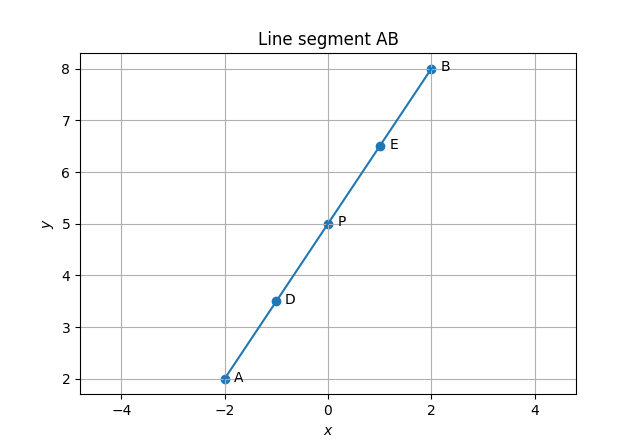
\includegraphics[scale=0.49]{Figure_1.png}
 
 \end{center}
Given Data:A = \myvec{-2\\2}\\
           B = \myvec{2\\8}\\
\\To find:C,D,E = ?\\

   let,k=1 
Now, 
\begin{align}
C = \frac{A+kB}{k+1}\\
C = \frac{\myvec{-2\\2}+1\myvec{2\\8}}{(1+1)}\\
= \frac{\myvec{-2\\2}+\myvec{2\\8}}{2}\\
= \frac{\myvec{0\\10}}{2}\\
 = \myvec{0\\5}\\
C = (0,5)
\end{align}	
now, 
\begin{align}
D = \frac{A+kC}{k+1}\\
D = \frac{\myvec{-2\\2}+1\myvec{0\\5}}{(1+1)}\\
= \frac{\myvec{-2\\2}+\myvec{0\\5}}{2}\\
= \frac{\myvec{-2\\7}}{2}\\
= \myvec{-1\\\frac{7}{2}}\\
D = (-1,\frac{7}{2})
\end{align}
Similarly,the third point 
\begin{align}
E = \frac{C+kB}{k+1}\\
E = \frac{\myvec{0\\5}+1\myvec{2\\8}}{(1+1)}\\
= \frac{\myvec{0\\5}+\myvec{2\\8}}{2}\\
= \frac{\myvec{2\\13}}{2}\\
 = \myvec{2\\\frac{13}{2}}\\
E = (2,\frac{13}{2})
\end{align}
therefore,the three points which divide AB into four equal parts are:\\
C = (0,5),
D = $(-1,\frac{7}{2})$,
E = $(2,\frac{13}{2})$
\end{enumerate}


\end{document}